\newpage
\section{Definizione del Prodotto}

\subsection{Metodo e formalismo di specifica}
Verrà qui esposta l'architettura di Premi ad alto livello seguendo un approccio top-down$_G$: verranno prima descritti i package$_G$ e le loro dipendenze e successivamente le singole classi contenute al loro interno. I diagrammi delle classi e dei package$_G$ seguono il formalismo UML$_G$2.0 e la struttura dei package segue una prassi ("best practice$_G$") di AngularJS$_G$ che propone una suddivisione dei componenti per funzionalità dell'applicazione in alternativa alla classica suddivisione Model-View-Controller$_G$, più difficile da mantenere per applicazioni di medie o grandi dimensioni. Per ulteriori approfondimenti consultare la guida al sito \href{https://scotch.io/tutorials/angularjs-best-practices-directory-structure}{scotch.io} oppure il tutorial di \href{http://angular-meteor.com/tutorial/step_07}{urigo:angular-meteor}.
Si illustreranno poi i Design Pattern utilizzati nella fase di progettazione ad alto livello e si descriveranno le interazioni dell'utente con l'applicazione attraverso i diagrammi di attività$_G$.


\subsection{Presentazione dell'architettura generale del sistema}

I componenti sono stati suddivisi prima in base al loro contributo a specifiche funzionalità del software e solo successivamente per appartenenza ai ruoli del pattern MVC$_G$. Questo aumenta la chiarezza espositiva dei diagrammi, evita la creazione di package$_G$ contenenti un numero eccessivo di classi e aiuta a compiere verifiche mirate a singoli componenti. \\
È importante specificare che il framework AngularJS$_G$ unisce view e controller attraverso una dichiarazione esterna a entrambi, che fa parte del meccanismo detto di \textit{routing} o di reindirizzamento dell'utente; view e controller inoltre non sanno di essere collegati tra loro e comunicano attraverso un oggetto chiamato \textit{\$scope}. Questo rende l'architettura sia di tipo Model-View-Controller$_G$ che di tipo Model-View-ViewModel$_G$. \\
Per motivi di leggibilità \$scope e routing non verranno rappresentati in modo esplicito nei diagrammi dei package e delle classi di questo documento, ma sono comunque da considerarsi impliciti nelle dipendenze tra i view e controller dei componenti. \\
\subsection{Server}

\begin{figure}[h]
\begin{center}
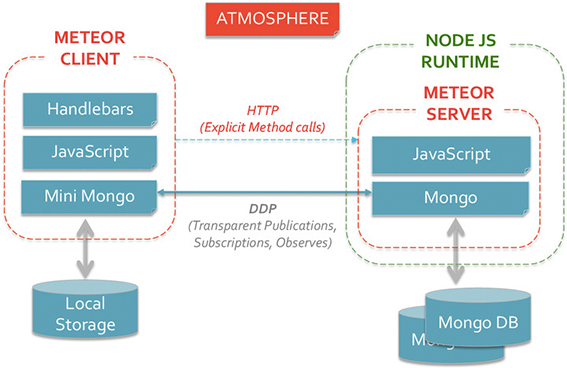
\includegraphics[scale=0.35]{img/meteor_architettura.jpg}
\caption{Schema archittetura}
\end{center}
\end{figure}

La comunicazione con la componente server avviene tramite la libreria Node.js$_G$ già implementata in MeteorJS$_G$. Con questa componente l'archittetura permette di realizzare un'applicazione asincrona, che a differenza del modello classico client-server permette di eseguire operazioni utili durante l'attesa di ricevere o di modificare un dato richiesto.
Nel server sono presenti delle funzioni che permettono al client di reperire i dati dal database MongoDB$_G$ residente nel server. In locale vengono scaricati solo i file richiesti che servono in quel momento. Ogni modifica al database viene effettuata prima in locale sul database minimongo$_G$. MeteorJS esegue in automatico in background la sincronizzazione tra il database locale minimongo$_G$ e tra il database server MongoDB$_G$.
\clearpage
\newpage
\section{Diagrammi dei Package}
Di seguito vengono descritti componenti principali del sistema e le loro dipendenze.

\begin{figure}[h]
\begin{center}
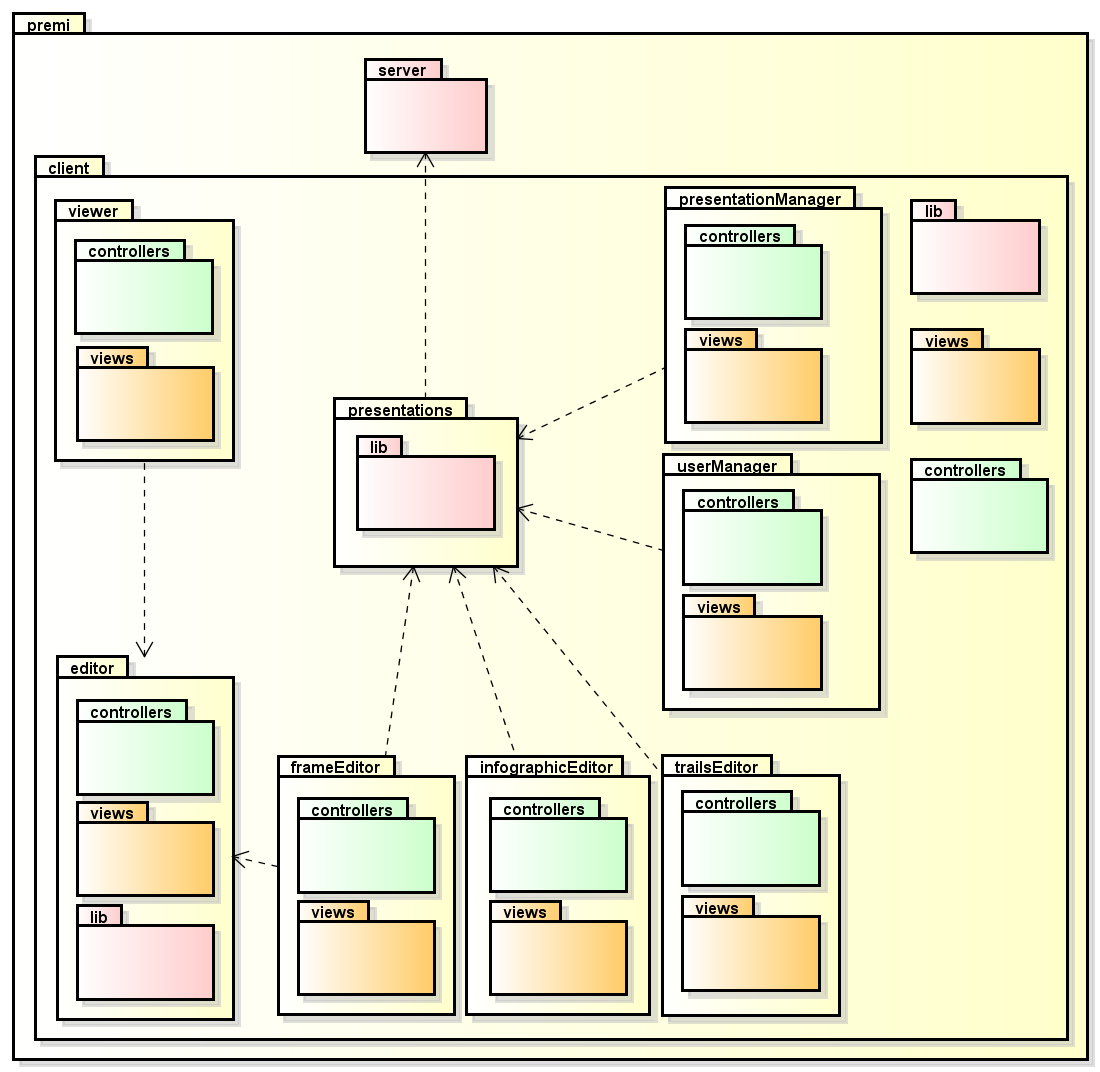
\includegraphics[scale=0.35]{img/diapkg/package.png}
\caption{Diagramma dei package di Premi.}
\end{center}
\end{figure}

L'applicazione è costituita da un solo package$_G$ principale chiamato \code{Premi}; oltre alla view ed al controller principali, al suo interno sono presenti:
\begin{itemize}
\item \code{premi.server} contiene una libreria di metodi per l'inserimento, l'aggiornament e la rimozione dei dati presenti nel database$_G$;
\item \code{premi.client} è il package principale che gestisce le funzionalità offerte all'utente;
\item \code{Premi.client.viewer} racchiude gli elementi necessari alla visualizzazione della presentazione nei vari contesti previsti(presentazione live, pubblica e privata);
\item \code{PrXXXXXXXXXXXXXXXXXemi.UserManager} è il package$_G$ di gestione dei dati dell'utente, contiene view e controller per la sua creazione e modifica, e la classe che lo definisce;
\item \code{PrXXXXXXXXXXXXXXXXXemi.Viewer} racchiude gli elementi necessari alla visualizzazione della presentazione nei vari contesti previsti(presentazione live, pubblica e privata);
\item \code{PrXXXXXXXXXXXXXXXXXemi.Presentation} racchiude la struttura generale della presentazione;
\item \code{PrXXXXXXXXXXXXXXXXXemi.PresentationManager} contiene gli elementi necessari alla gestione delle presentazioni da parte dell'utente;
\item \code{PrXXXXXXXXXXXXXXXXXemi.Editor} è il package$_G$ dedicato alla modifica interna delle presentazioni; possiede al suo interno tre ulteriori package$_G$:
\begin{itemize}
\item \code{PrXXXXXXXXXXXXXXXXXemi.Editor.FrameEditor} si occupa di creare, modificare o cancellare i Frame$_G$ contenuti nella presentazione;
\item \code{PrXXXXXXXXXXXXXXXXXemi.Editor.InfographicEditor} posiziona Frame$_G$ o altri elementi all'interno di un poster;
\item \code{PrXXXXXXXXXXXXXXXXXemi.Editor.TrailsEditor} ordina i Frame per la creazione di uno o più percorsi di presentazione.
\end{itemize}
\end{itemize}

\clearpage